\section{Life course of intimate relationships}

Levy \cite{levy2014intimate} has defined a so called \textit{life course of intimate relationships}. This course includes four conditions of romantic relationships (see Figure \ref{fig:live_course}). Each condition is colored from colors from figure \ref{fig:cluster}. Here, the connection to the individual topics should be roughly indicated. The transitions in content are sometimes fluid.
\begin{figure}[htb]
    \centering
	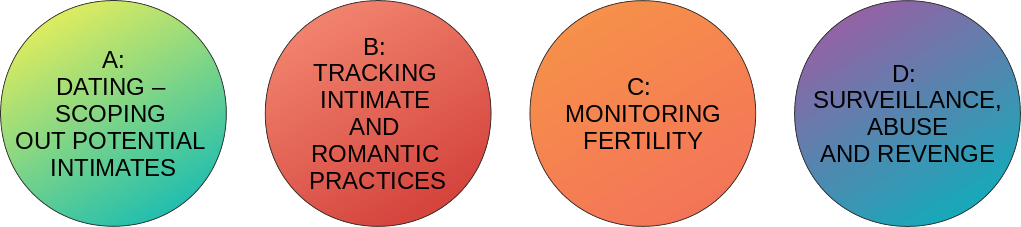
\includegraphics[width=\linewidth]{img/life_course_of_intimate_surveillance.png}
	\caption{The life course of intimate surveillance. Each condition is co}
	\label{fig:live_course}
\end{figure}

In each of these conditions (potential) partners can use technologies for different purposes.

Condition \textbf{A} stands for the beginning of a potential relationship. The partners know each other or would like to know each other. At this point, there is an interest from one or both sides. The aim is to learn more about the other person, to check their identity and social life.

In condition \textbf{B} the partners are already in a relationship or something appropriate. At this point, it should be emphasized that this condition includes all sorts of relationships that are understood as such. For a concretely definition what a (romantic) relationship means see Danaher et al. \cite{doi:10.1080/15265161.2017.1409823} or \ref{sec:terms_of_definition}. In this condition the partners know each other better and have an increased (mutual) interest. There were other forms of contact, possibly sexual contact.

In condition \textbf{C} there is usually an established relationship (but that does not have to be the case, there maybe exceptions). The couple exercises sexual activities, deals with contraceptive measures (together) or plans to start a family.

Condition \textbf{D} contains the surveillance of the partner, also abuse (of data) and revenge. Describing this condition is complicate. 
It can be a relationship that has already ended. The partners therefore have a relationship to each other based on their previous history. This can be different (as in the other states). More generally, this condition maybe arise from problems in the relationship, due to interpersonal conflicts oder something else. But it may also be a state or point in the relationship which is fine for both partner (that refers to the surveillance). This will be discussed later on.

Since relationships are complex and individual, the single conditions are not interconnected \cite{sassler2010partnering}. Also this is not the focus of this work. The descriptions above only should give an idea of what the conditions mean for the following section \ref{sec:consideration_life_course_conditions}, in which all conditions will be discussed in detail.
